% Options for packages loaded elsewhere
\PassOptionsToPackage{unicode}{hyperref}
\PassOptionsToPackage{hyphens}{url}
\PassOptionsToPackage{dvipsnames,svgnames,x11names}{xcolor}
%
\documentclass[
  sn-basic,
]{sn-jnl}



\usepackage{amsmath,amssymb}
\usepackage{iftex}
\ifPDFTeX
  \usepackage[T1]{fontenc}
  \usepackage[utf8]{inputenc}
  \usepackage{textcomp} % provide euro and other symbols
\else % if luatex or xetex
  \usepackage{unicode-math}
  \defaultfontfeatures{Scale=MatchLowercase}
  \defaultfontfeatures[\rmfamily]{Ligatures=TeX,Scale=1}
\fi
\usepackage{lmodern}
\ifPDFTeX\else  
    % xetex/luatex font selection
\fi
% Use upquote if available, for straight quotes in verbatim environments
\IfFileExists{upquote.sty}{\usepackage{upquote}}{}
\IfFileExists{microtype.sty}{% use microtype if available
  \usepackage[]{microtype}
  \UseMicrotypeSet[protrusion]{basicmath} % disable protrusion for tt fonts
}{}
\makeatletter
\@ifundefined{KOMAClassName}{% if non-KOMA class
  \IfFileExists{parskip.sty}{%
    \usepackage{parskip}
  }{% else
    \setlength{\parindent}{0pt}
    \setlength{\parskip}{6pt plus 2pt minus 1pt}}
}{% if KOMA class
  \KOMAoptions{parskip=half}}
\makeatother
\usepackage{xcolor}
\setlength{\emergencystretch}{3em} % prevent overfull lines
\setcounter{secnumdepth}{5}
% Make \paragraph and \subparagraph free-standing
\makeatletter
\ifx\paragraph\undefined\else
  \let\oldparagraph\paragraph
  \renewcommand{\paragraph}{
    \@ifstar
      \xxxParagraphStar
      \xxxParagraphNoStar
  }
  \newcommand{\xxxParagraphStar}[1]{\oldparagraph*{#1}\mbox{}}
  \newcommand{\xxxParagraphNoStar}[1]{\oldparagraph{#1}\mbox{}}
\fi
\ifx\subparagraph\undefined\else
  \let\oldsubparagraph\subparagraph
  \renewcommand{\subparagraph}{
    \@ifstar
      \xxxSubParagraphStar
      \xxxSubParagraphNoStar
  }
  \newcommand{\xxxSubParagraphStar}[1]{\oldsubparagraph*{#1}\mbox{}}
  \newcommand{\xxxSubParagraphNoStar}[1]{\oldsubparagraph{#1}\mbox{}}
\fi
\makeatother


\providecommand{\tightlist}{%
  \setlength{\itemsep}{0pt}\setlength{\parskip}{0pt}}\usepackage{longtable,booktabs,array}
\usepackage{calc} % for calculating minipage widths
% Correct order of tables after \paragraph or \subparagraph
\usepackage{etoolbox}
\makeatletter
\patchcmd\longtable{\par}{\if@noskipsec\mbox{}\fi\par}{}{}
\makeatother
% Allow footnotes in longtable head/foot
\IfFileExists{footnotehyper.sty}{\usepackage{footnotehyper}}{\usepackage{footnote}}
\makesavenoteenv{longtable}
\usepackage{graphicx}
\makeatletter
\newsavebox\pandoc@box
\newcommand*\pandocbounded[1]{% scales image to fit in text height/width
  \sbox\pandoc@box{#1}%
  \Gscale@div\@tempa{\textheight}{\dimexpr\ht\pandoc@box+\dp\pandoc@box\relax}%
  \Gscale@div\@tempb{\linewidth}{\wd\pandoc@box}%
  \ifdim\@tempb\p@<\@tempa\p@\let\@tempa\@tempb\fi% select the smaller of both
  \ifdim\@tempa\p@<\p@\scalebox{\@tempa}{\usebox\pandoc@box}%
  \else\usebox{\pandoc@box}%
  \fi%
}
% Set default figure placement to htbp
\def\fps@figure{htbp}
\makeatother

%%%% Standard Packages

\usepackage{graphicx}%
\usepackage{multirow}%
\usepackage{amsmath,amssymb,amsfonts}%
\usepackage{amsthm}%
\usepackage{mathrsfs}%
\usepackage[title]{appendix}%
\usepackage{xcolor}%
\usepackage{textcomp}%
\usepackage{manyfoot}%
\usepackage{booktabs}%
\usepackage{algorithm}%
\usepackage{algorithmicx}%
\usepackage{algpseudocode}%
\usepackage{listings}%

%%%%

\raggedbottom
\makeatletter
\@ifpackageloaded{caption}{}{\usepackage{caption}}
\AtBeginDocument{%
\ifdefined\contentsname
  \renewcommand*\contentsname{Table of contents}
\else
  \newcommand\contentsname{Table of contents}
\fi
\ifdefined\listfigurename
  \renewcommand*\listfigurename{List of Figures}
\else
  \newcommand\listfigurename{List of Figures}
\fi
\ifdefined\listtablename
  \renewcommand*\listtablename{List of Tables}
\else
  \newcommand\listtablename{List of Tables}
\fi
\ifdefined\figurename
  \renewcommand*\figurename{Figure}
\else
  \newcommand\figurename{Figure}
\fi
\ifdefined\tablename
  \renewcommand*\tablename{Table}
\else
  \newcommand\tablename{Table}
\fi
}
\@ifpackageloaded{float}{}{\usepackage{float}}
\floatstyle{ruled}
\@ifundefined{c@chapter}{\newfloat{codelisting}{h}{lop}}{\newfloat{codelisting}{h}{lop}[chapter]}
\floatname{codelisting}{Listing}
\newcommand*\listoflistings{\listof{codelisting}{List of Listings}}
\usepackage{amsthm}
\theoremstyle{plain}
\newtheorem{theorem}{Theorem}[section]
\theoremstyle{plain}
\newtheorem{proposition}{Proposition}[section]
\theoremstyle{remark}
\AtBeginDocument{\renewcommand*{\proofname}{Proof}}
\newtheorem*{remark}{Remark}
\newtheorem*{solution}{Solution}
\newtheorem{refremark}{Remark}[section]
\newtheorem{refsolution}{Solution}[section]
\makeatother
\makeatletter
\makeatother
\makeatletter
\@ifpackageloaded{caption}{}{\usepackage{caption}}
\@ifpackageloaded{subcaption}{}{\usepackage{subcaption}}
\makeatother

\usepackage{bookmark}

\IfFileExists{xurl.sty}{\usepackage{xurl}}{} % add URL line breaks if available
\urlstyle{same} % disable monospaced font for URLs
\hypersetup{
  pdftitle={Tail Flexibility in the Degrees of Preferential Attachment Networks},
  pdfauthor={Thomas William Boughen; Clement Lee; Vianey Palacios Ramirez},
  pdfkeywords={networks, discrete extremes, power law, preferential
attachment},
  colorlinks=true,
  linkcolor={blue},
  filecolor={Maroon},
  citecolor={Blue},
  urlcolor={Blue},
  pdfcreator={LaTeX via pandoc}}


\title[Tail Flexibility in the Degrees of Preferential Attachment
Networks]{Tail Flexibility in the Degrees of Preferential Attachment
Networks}

% author setup
\author[1]{\fnm{Thomas William} \sur{Boughen}}\author[1]{\fnm{Clement} \sur{Lee}}\author[1]{\fnm{Vianey Palacios} \sur{Ramirez}}
% affil setup
\affil[1]{\orgdiv{School of Mathematics, Statistics and
Physics}, \orgname{Newcastle University}}

% abstract 

\abstract{Devising the underlying generating mechanism of a real-life
network is difficult as, more often than not, only its snapshots are
available, but not its full evolution. One candidate for the generating
mechanism is preferential attachment which, in its simplest form,
results in a degree distribution that follows the power law.
Consequently, the growth of real-life networks that roughly display such
power-law behaviour is commonly modelled by preferential attachment.
However, the validity of the power law has been challenged by the
presence of alternatives with comparable performance, as well as the
recent findings that the right tail of the degree distribution is often
lighter than implied by the body, whilst still being heavy. In this
paper, we study a modified version of the model with a flexible
preference function that allows super/sub-linear behaviour whilst also
guaranteeing that the limiting degree distribution has a heavy tail. We
relate the distributions tail heaviness directly to the model
parameters, allowing direct inference of the parameters from the degree
distribution alone.}

% keywords
\keywords{networks,  discrete extremes,  power law,  preferential
attachment}

\begin{document}
\maketitle


\newpage

\section{Introduction}\label{introduction}

Networks appear in many fields such as sociology, politics,
epidemiology, and economics. Statistical methods have been and continue
to be used to study networks that appear in these fields and beyond,
from the use of stochastic block models to detect communities within the
French political blogosphere \citep{Latouche11}, to using Exponential
Random Graph Models (ERGMs) to analyse the global trade network
\citep{Setayesh22}, and the use of mechanistic models in neuroscience to
investigate the patterns of connections in neural systems
\citep{Betzel17}.

One example of a mechanistic model that may be considered is the
preferential attachment (PA) model where as a network grows and new
vertices join they connect to those already present in the network with
weights proportional to some preference function \(b(\cdot)\) of their
in-degree. The well-known Barabási-Albert (BA) model is a special case
of this when \(b(k) = k+1\) \citep{Barabasi99}.

These mechanistic models are generally useful when simulating networks,
but not for fitting to real data as usually only snapshots of a network
are available and not the full evolution - without this conclusions
about the growth are difficult to make. However, one statistic that is
usually available for snapshots of networks is the degree distribution
making it valuable to study the degrees in a network. Often, when
looking at the degree distributions of real networks it can be
attractive to use the power law \footnote{Power law:
  \(\bar F(k) = L(k)\cdot k^{-1/\xi}\), where \(\xi>0\) and \(L(k)\) is
  slowly varying in \(k\).} when modelling as it is seemingly observed
in much of the data. It also comes with the added benefit of offering a
connection to preferential attachment since the BA model results in a
power law degree distribution \citep{Barabasi99}, perhaps suggesting
that if the power law fits well then the network may have grown
according to similar simple rules. However, attempting to explain the
networks growth using preferential attachment when the degrees seemingly
follow a power law may not be the best course of action as
\citep{krapivsky01} shows that a general preference function does not
necessarily lead to power law degrees, showing that a preference
function of form \(b(k) = k^\alpha\) leads to light tails when
\(\alpha<1\), a degenerate network (a finite number of vertices end up
with all of the added edges) when \(\alpha>1\), and only yielding heavy
tails when \(\alpha=1\). Additionally, it is still being argued whether
or not a lot of real data actually follows a power law.
\citet{Broido_2019} provides some evidence that suggests that real world
networks rarely have degrees that follow a power law through the use of
statistical analysis of almost 1000 networks across a wide variety of
fields; \citet{Voitalov_2019}, on the other hand, disagrees and claims
that these kinds of networks are not nearly as rare and only appear so
as a result of an unrealistic expectation of power law without
deviations or noise. \citet{rudas07} derives the limiting degree
distribution in terms of the preference function \(b(\cdot)\) and its
parameters, we build upon this by finding a class of preference
functions that result in realistic tails i.e.~heavy but not as heavy as
implied by the power law.

Extreme value methods have been scarcely used when it comes to analysis
of degree distributions and whether they follow the power law. The
absence of these methods essentially down weights the deviation of
vertices with the largest degrees, which are usually the most
influential, from the power law. Somewhat recent publications
\citep{Voitalov_2019, Lee24, wang2022random} have addressed this gap in
the literature. \citet{Voitalov_2019} proposes estimating the power law
exponent of a degree distribution using three estimators based in
extreme value theory, in contrast to the estimators generally used in
network science, the degree distributions are then split into one of
three categories (not power-law , hardly power-law or power-law)
depending on the values of the estimates obtained from each of the
estimators. \citet{Lee24} proposes a framework for modelling entire
degree distributions using a combination of two generalisations of the
power law including a model selection step that is capable of suggesting
whether or not the data is adequately modelled by a power law, with one
conclusion being that most data seems to have a tail lighter than what
is implied by the body whilst still being heavy tailed.
\citet{wang2022random} considers a preferential attachment model with an
affine preference function and reciprocal edges, they study the limiting
degree distribution of this model for both the in-degrees and
out-degrees - finding that the joint limiting distribution is
multivariate regularly varying and has the property of hidden regular
variation.

Evidently, the study of degree distributions is a very active but the
vast majority of research in the field (whether using extremes or not)
are purely descriptive in the sense that no information about the
preference function is revealed even if preferential attachment was the
underlying mechanism. This paper aims to address this gap - asking if
given the degree distribution of a network assumed to come from the
preferential attachment model, can we directly infer the model
parameters?

The remainder of this paper begins with a more detailed description of
the PA model alongside the theoretical results for the limiting degree
distribution using results from \citet{rudas07},
(Section~\ref{sec-tail}) then goes on to analyse the tail behaviour of
this limiting distribution in terms of the preference function
\(b(\cdot)\) arguing that a heavy tailed degree distribution can only be
the result of an asymptotically linear preference function shown by
Proposition~\ref{prp-omega} - ending with a suggestion for a preference
function that can guarantee heavy tails while remaining flexible.
Section~\ref{sec-model} builds on the results from
Section~\ref{sec-tail} and considers the limiting distribution obtained
when using a preference function of the form stated at the end of
Section~\ref{sec-tail} providing examples of how the shape of the
distribution varies with respect to the model parameters as well as
visualisations for how the tail heaviness changes when these parameters
are varied - continued study of this distribution then also reveals a
connection to the general Pareto distribution (GPD).
Section~\ref{sec-sim} consists of a simulation study where networks are
simulated from the PA model for various parameter combinations and then
the model specified in Section~\ref{sec-model} is fitted to the
resulting degree distributions using Bayesian inference, demonstrating
that (for simulated data) the model parameters can be recovered from
only the degree distribution. Finally, Section~\ref{sec-real} fits the
model to some real data and provides posterior estimates for the
preference function assuming the networks evolved according to the PA
model.

\newpage

\section{Tail Behaviour of Preferential Attachment
Model}\label{sec-tail}

The network generative model that we will be focussing on in this paper
is dubbed General Preferential Attachment in \citep{rudas07} and is
defined as follows:

Starting at time \(t=0\) with an initial network of \(m\) vertices that
each have no edges, at times \(t=1,2,\ldots\) a new vertex is added to
the network bringing with it \(m\) directed edges (with the new vertex
as the source); the target for each of these edges are selected from the
vertices already in the network with weights proportional to some
function \(b\) of their degree where the preference function \(b\) is
chosen such that:

\begin{equation}\phantomsection\label{eq-condb1}{
b:\mathbb N \mapsto \mathbb R^+\setminus\{0\},
}\end{equation}

\begin{equation}\phantomsection\label{eq-condb2}{
\sum_{k=0}^\infty\frac{1}{b(k)} = \infty.
}\end{equation}

Special cases of this model include the Barabási-Albert (BA) model when
\(b(k) = k+\varepsilon\), which leads to a power-law degree distribution
with \(\xi=1/2\) and the Uniform Attachment (UA) model where \(b(k)=c\)
leading to a degree distribution that is light tailed.

Given conditions \ref{eq-condb1} and \ref{eq-condb2} an expression for
the survival of the limiting degree distribution can be found in the
case that \(m=1\); obtained by considering a branching process that is
equivalent to the growth of the network, as in \citep{rudas07}. Theorem
1 from \citep{rudas07} states that for the tree \(\Upsilon(t)\) at time
\(t\):

\begin{equation}\phantomsection\label{eq-survlim}{
\lim_{t\rightarrow\infty}\frac{1}{|\Upsilon(t)|}\sum_{x\in\Upsilon(t)}\varphi(\Upsilon(t)_{\downarrow x}) = \lambda^* \int_0^\infty e^{-\lambda^* t}\mathbb E\left[\varphi(\Upsilon(t))\right]dt
}\end{equation} where \(\lambda^*\) satisfies \(\hat\rho(\lambda^*)=1\).

The limiting survival can be viewed as the limit of the empirical
proportion of vertices with degree over a threshold \(k\), that is:

\[
\bar F(k) = \lim_{t\rightarrow\infty}\frac{\sum_{x\in\Upsilon(t)}\mathbb I\left\{\text{deg}(x,\Upsilon(t)_{\downarrow x})>k\right\}}{\sum_{x\in\Upsilon(t)} 1}
\] which can also be written using Equation~\ref{eq-survlim} as:

\[
\bar F(k) = \frac{\int_0^\infty e^{-\lambda^* t}\mathbb E\left[\mathbb I\left\{\text{deg}(x,\Upsilon(t))>k\right\}\right]dt}{\int_0^\infty e^{-\lambda^* t}dt} = \prod_{i=0}^k\frac{b(i)}{\lambda^* + b(i)}
\] Additionally, using the fact that \(f(k) = \bar F(k-1) - \bar F(k)\)
the limiting degree distribution can be shown to be:

\[
f(k) = \frac{\lambda^*}{\lambda^* + b(k)}\prod_{i=0}^{k-1}\frac{b(i)}{\lambda^*+b(i)},\qquad k\in\mathbb N.
\]

We are interested in how the tail behaviour of the limiting degrees is
affected by the preference function \(b\).

\citep{shimura12} introduces a quantity that will help in determining
this for this discrete distribution, that is:

For a distribution \(F\) with survival function \(\bar F\) and some
\(k\in\mathbb Z^+\) let:

\[
\Omega(F,k) = \left(\log\displaystyle\frac{\bar F (k+1)}{\bar F (k+2)}\right)^{-1} - \left(\log\displaystyle\frac{\bar F (k)}{\bar F (k+1)}\right)^{-1}
\]

\citep{shimura12} then states that if
\(\lim_{n\rightarrow\infty} \Omega(F,k) = 1/\alpha\) (\(\alpha>0\)),
then \(F\) is heavy tailed with \(\bar F(k) \sim k^{-\alpha}\).
Additionally, if \(\lim_{n\rightarrow\infty} \Omega(F,k) = 0\) then the
distribution is light tailed. This allows us to show the following:

\begin{proposition}[]\protect\hypertarget{prp-omega}{}\label{prp-omega}

If \(b(k) \rightarrow \infty\) as \(k\rightarrow \infty\) then \[
\bar F(k) = \prod_{i=0}^k\frac{b(i)}{\lambda^* + b(i)}
\] and

\[
\lim_{k\rightarrow\infty}\Omega(F,k) = \lim_{k\rightarrow\infty}\frac{b(k+1)-b(k)}{\lambda^*}.
\]

\end{proposition}

See appendix \ref{sec-proofs} for the details of the proof.

Proposition~\ref{prp-omega} aligns with the result from
\citep{krapivsky01} demonstrating that a sub-linear preference function
will lead to a light tailed distribution. So, in order for the degree
distribution to be heavy tailed we need that the limit
\(\lim_{k\rightarrow\infty} b(k+1)-b(k)\) exists and is positive. We can
in fact show that BA model produces a heavy tailed degree distribution
with index \(\xi=0.5\) by considering the preference function
\(b(k) = k + \varepsilon\), noting that the limit
\(\lim_{k\rightarrow\infty} b(k+1)-b(k)\) is simply
\(\lim_{k\rightarrow\infty} 1 = 1\) leaving the tail heaviness to be
\(1/\lambda^*\) which using \(\hat\rho\) can be found to be \(1/2\).

\begin{theorem}[Stolz-Cesàro Theorem
\citep{cesaro}]\protect\hypertarget{thm-stolz}{}\label{thm-stolz}

Let \((a_n)_{n\ge1}\) and \((b_n)_{n\ge1}\) be two sequence of real
numbers. Assume \((a_n)_{n\ge1}\) is a strictly monotone and divergent
sequence and the following limit exists:

\[
\lim_{k\rightarrow\infty}\frac{b_{k+1} - b_k}{a_{k+1} - a_k} = l.
\] Then,

\[
\lim_{k\rightarrow\infty}\frac{b_k}{a_k} = l.
\]

\end{theorem}

\begin{proposition}[]\protect\hypertarget{prp-omega2}{}\label{prp-omega2}

Consider a GPA model with preference function \(b(\cdot)\) satisfying
Proposition~\ref{prp-omega}. If
\(\lim_{k\rightarrow\infty}\frac{b(k)}{k} = c\), then the limiting
degree distribution has a heavy tail with index \(c\over\lambda^*\) and
this heavy tail may only be the result of a preference function of this
form (asymptotically linear).

\emph{Proof}

From Proposition~\ref{prp-omega}, we have that: \[
\lim_{k\rightarrow\infty}[b(k+1)-b(k)] = c>0.
\] Now, setting \(b_k = b(k)\) and \(a_k = k\):

\[
\lim_{k\rightarrow\infty}[b(k+1)-b(k)] = \lim_{k\rightarrow\infty}\frac{b_{k+1} - b_k}{a_{k+1} - a_k} = c>0,
\] meaning by Theorem~\ref{thm-stolz}:

\[
\lim_{k\rightarrow\infty}\frac{b_k}{a_k} = \lim_{k\rightarrow\infty}\frac{b(k)}{k} = c>0\qquad \square.
\]

\end{proposition}

Considering Proposition~\ref{prp-omega2} we propose the following
preference function:

\[
b(k) = \begin{cases}
k^\alpha + \varepsilon,&k<k_0\\
k_0^\alpha + \varepsilon + \beta(k-k_0), &k\ge k_0
\end{cases}
\] for \(\alpha,\beta, \varepsilon>0\) and \(k_0\in\mathbb N\).

This preference function, as per Proposition~\ref{prp-omega}, will
produce a degree distribution with tail heaviness \(\beta/\lambda^*\)
guaranteeing a heavy tail. We study this preference function further in
the next section.

\newpage

\section{Preferential Attachment with Flexible Heavy
Tail}\label{sec-model}

Using a preference function with guaranteed linear behaviour in the
limit, allows for the inclusion of sub/super linear behaviour without
losing the heavy tails or ending up with a degenerate degree
distribution.

The limiting degree distribution resulting from using a preference
function of this form can be found to have survival:

\begin{equation}\phantomsection\label{eq-polysurv}{
\bar F(k) = \begin{cases}
\prod_{i=0}^{k}\frac{i^\alpha + \varepsilon}{\lambda^*+i^\alpha + \varepsilon},&k<k_0\\
\left(\prod_{i=0}^{k_0-1}\frac{i^\alpha + \varepsilon}{\lambda^*+i^\alpha + \varepsilon}\right)\frac{\Gamma(\lambda^*+k_0^\alpha + \varepsilon)/\beta)}{\Gamma\left((k_0^\alpha + \varepsilon)/\beta\right)} \frac{\Gamma\left(k-k_0 + 1 +\frac{k_0^\alpha + \varepsilon}{\beta}\right)}{\Gamma\left(k-k_0 + 1 +\frac{\lambda^* +k_0^\alpha + \varepsilon}{\beta}\right)},&k\ge k_0.
\end{cases}
}\end{equation}

with \(\lambda^*\) satisfying \(\hat \rho(\lambda^*)=1\) where:

\begin{equation}\phantomsection\label{eq-rho}{
\hat\rho(\lambda) = \sum_{n=0}^{k_0}\prod_{i=0}^{n-1}\frac{i^\alpha + \varepsilon}{\lambda+i^\alpha + \varepsilon} + \left(\frac{k_0^\alpha + \varepsilon}{\lambda-\beta}\right)\prod_{i=0}^{k_0-1}\frac{i^\alpha + \varepsilon}{\lambda + i^\alpha + \varepsilon} 
}\end{equation}

which must be solved numerically for most parameter choices. Also, note
that \(\lambda>\beta\).

Some examples of what the degree distribution looks like for various
parameters are shown below in Figure~\ref{fig-polylinsurv}:

\begin{figure}

\centering{

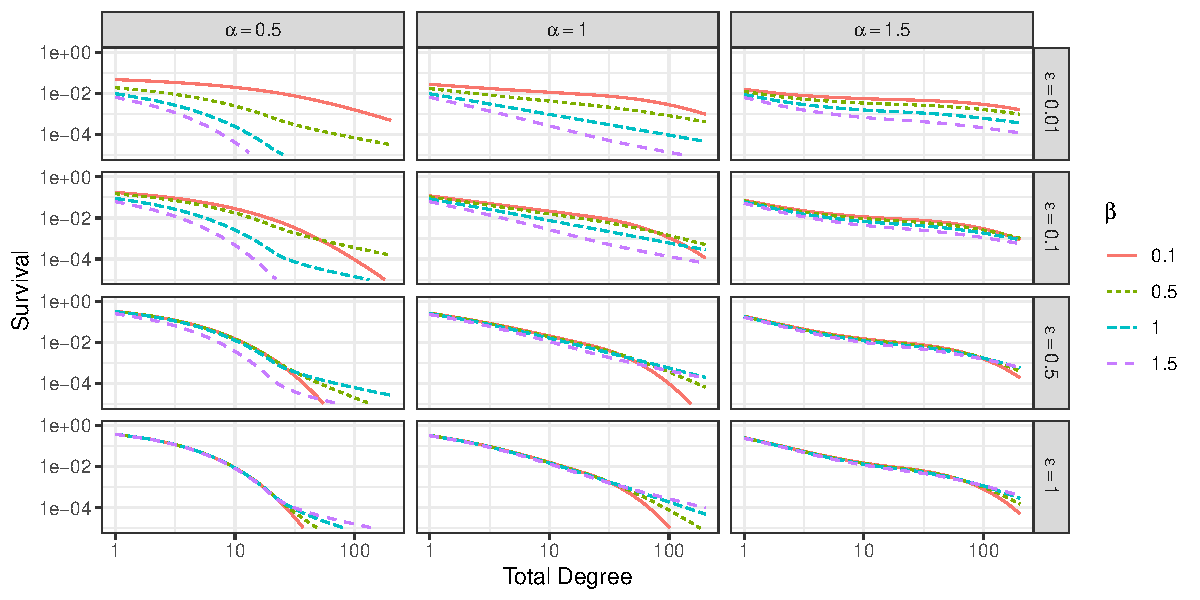
\includegraphics[width=0.8\linewidth,height=\textheight,keepaspectratio]{paper_files/figure-pdf/fig-polylinsurv-1.pdf}

}

\caption{\label{fig-polylinsurv}Theoretical survival distributions of
the limiting degree distributions, according to various combinations of
\((\alpha, \beta, \varepsilon)\) and \(k_0=20\) of the proposed
preferential attachment model.}

\end{figure}%

The survival function (\ref{eq-polysurv}) can be connected to a
discretised variation of the generalised Pareto distribution (GPD)
usually dubbed the Integer GPD (IGPD) with survival: \[
\Pr(X> x|X> v) = \left(\frac{\xi(x-v)}{\sigma} + 1\right)^{-1/\xi},\qquad x=v+1,v+2,\ldots
\] for \(v\in\mathbb Z^+, \sigma>0,\xi\in \mathbb R\), denoted as
\(X|X>u \sim  \mathrm {IGPD}(\xi, \sigma, u)\) where \(\xi\) is the
shape parameter controlling th tail heaviness.

By Equation~\ref{eq-polysurv} and using Stirling's approximation:

\begin{align*}
\bar F(k|k\ge k_0) &= \frac{\Gamma\left(\frac{\lambda^* + k_0^\alpha + \varepsilon}{\beta}\right)}{\Gamma\left(\frac{k_0^\alpha + \varepsilon}{\beta}\right)}\times\frac{\Gamma\left(k-k_0  +1 + \frac{k_0^\alpha + \varepsilon}{\beta}\right)}{\Gamma\left(k-k_0  +1 + \frac{\lambda^*+ k_0^\alpha + \varepsilon}{\beta}\right)}\\
&\approx\left(\frac{k_0^\alpha+\varepsilon}{\beta}\right)^{\lambda^*/\beta}\left(k-k_0+1+\frac{k_0^\alpha + \varepsilon}{\beta}\right)^{-\lambda^*/\beta}\\
&=\left(\frac{k_0^\alpha+\varepsilon}{k_0^\alpha+\varepsilon + \beta}\right)^{\lambda^*/\beta}\left(\frac{\beta(k-k_0)}{\beta + k_0^\alpha+\varepsilon} + 1\right)^{-\lambda^*/\beta}\\
&=\left(\frac{\beta(k+1-k_0)}{k_0^{\alpha}+\varepsilon} + 1\right)^{-\lambda^{*}/\beta}
\end{align*}

\[
\bar F(k) 
\begin{cases}
=\prod_{i=0}^{k}\frac{i^\alpha + \varepsilon}{\lambda^*+i^\alpha + \varepsilon},&k<k_0,\\
\approx \left(\prod_{i=0}^{k_0-1}\frac{i^\alpha + \varepsilon}{\lambda^*+i^\alpha + \varepsilon}\right) \left(\frac{\beta(k+1-k_0)}{k_0^{\alpha}+\varepsilon} + 1\right)^{-\lambda^*/\beta},&k\ge k_0,
\end{cases}
\] meaning that for \(k\ge k_0\) the limiting degree distribution (for
large \(k_0^\alpha\)) is approximated by
\(\text{IGPD}\left(\frac{\beta}{\lambda^*}, \frac{k_0^\alpha + \varepsilon}{\lambda^*},k_0-1\right)\).

To assess how close of an approximation this is, the theoretical
conditional survivals are shown in Figure~\ref{fig-approx_surv} in
colour and their IGPD approximations are shown in grey. The
approximation seems to hold up fairly well even for large degrees.

\begin{figure}

\centering{

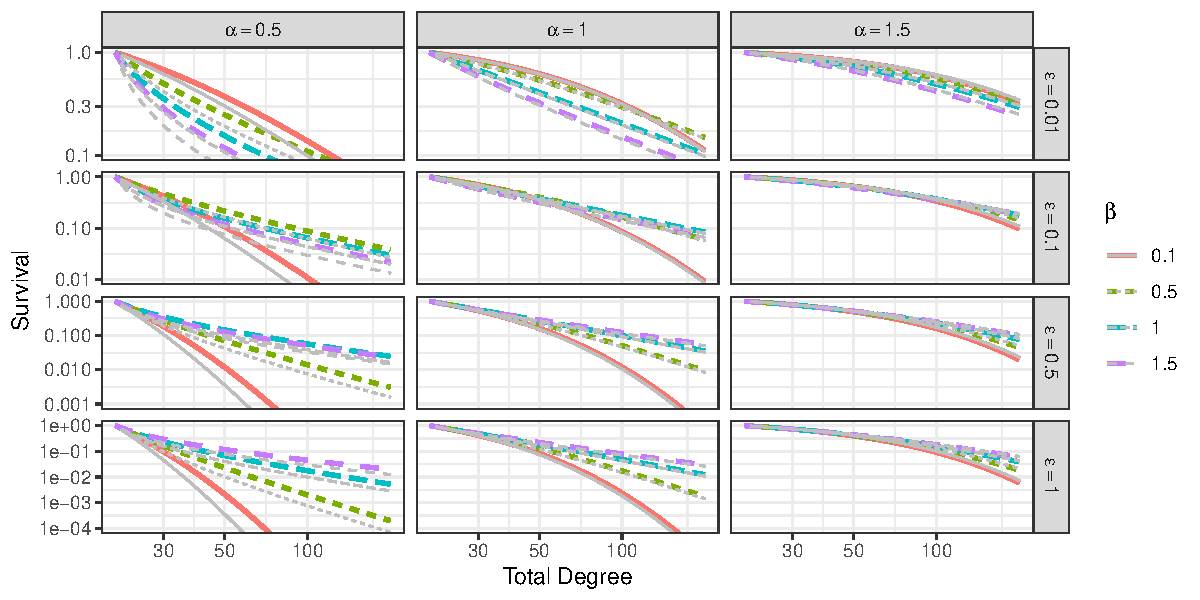
\includegraphics[width=0.8\linewidth,height=\textheight,keepaspectratio]{paper_files/figure-pdf/fig-approx_surv-1.pdf}

}

\caption{\label{fig-approx_surv}Theoretical conditional survivals (grey)
alongside their IGPD approximations (coloured).}

\end{figure}%

In agreement with Proposition~\ref{prp-omega2}, \(\beta>0\), the shape
parameter of the IGPD is positive and thus the distribution is heavy
tailed. Additionally the value of the shape parameter \(\xi\) is shown
in Figure~\ref{fig-polyheat} for various parameter choices. The darker
regions on the heat maps correspond to a heavier tail and the lighter to
a lighter tail, the red dashed line shows combinations of \(\alpha\) and
\(\beta\) that produce a limiting degree distribution with the same tail
heaviness as the Barabási-Albert model, \(\xi=0.5\).

\begin{figure}

\centering{

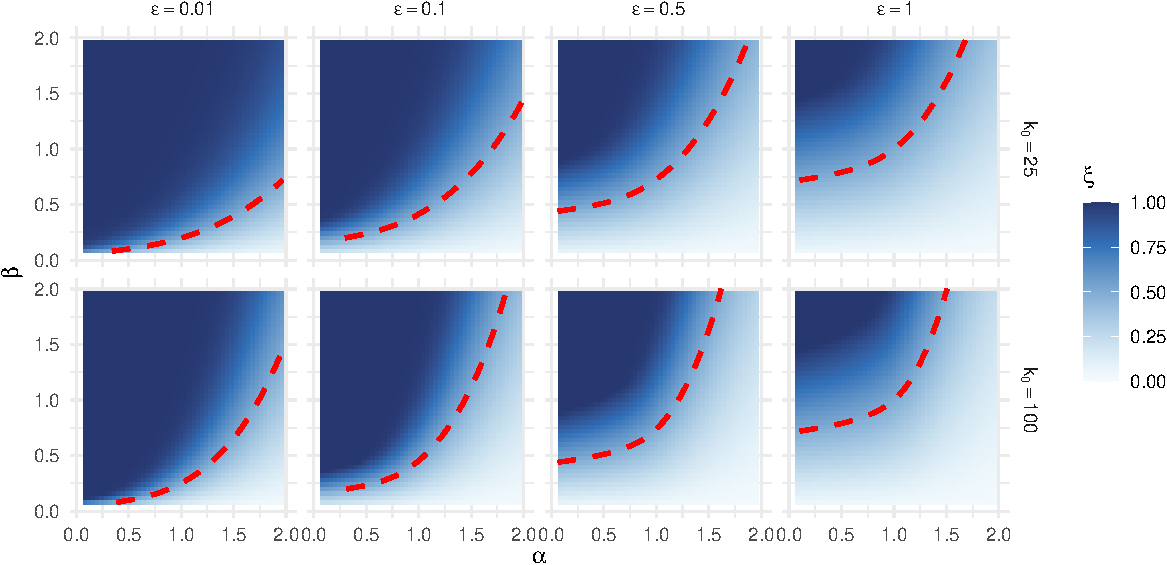
\includegraphics[width=0.8\linewidth,height=\textheight,keepaspectratio]{paper_files/figure-pdf/fig-polyheat-1.pdf}

}

\caption{\label{fig-polyheat}Heat maps of \(\xi\) for various
combinations of the parameters of the proposed model.}

\end{figure}%

Finally to be able to perform inference of the model parameters, we
consider a network with degree count vector
\(\pmb n = (n_0, n_1, \ldots, n_M)\) and maximum degree \(M\). We can
then write the likelihood of this model for this network as:

\begin{align*}
L(\pmb x,\pmb n | \pmb \theta) = \left(\frac{\lambda^*}{\lambda^*+\varepsilon}\right)^{n_0}\left(\prod_{j=l}^{k_0-1}\frac{j^\alpha +\varepsilon}{\lambda^* + j^\alpha +\varepsilon}\right)^{\left(\sum_{i\ge k_0}n_{i}\right)} \prod_{l \le i<k_0}\left(\frac{\lambda^*}{\lambda^* +i^\alpha + \varepsilon } \prod_{j=l}^{k_0-1}\frac{j^\alpha + \varepsilon}{\lambda^* + j^\alpha + \varepsilon}\right)^{n_i}\\ \times \prod_{i\ge k_0}\left(\frac{\text{B}(i-k_0 + (k_0^\alpha + \varepsilon)/\beta,1+\lambda^*/\beta)}{\text{B}((k_0^\alpha + \varepsilon)/\beta,\lambda^*/\beta)}\right)^{n_i}
\end{align*}

where \(B(y,z)\) is the the beta function and \(l\ge0\) is a variable
that allows truncating the data such that the minimum degree is \(l\),
which will allow the model to be fitted whilst ignoring the influence of
the lower degrees (those less than \(l\)) as the model does not capture
the behaviour at the lower degrees since \citet{rudas07} only provides
results for the case of a preferential attachment tree.

\section{Simulation Study}\label{sec-sim}

This section aims to show that the parameters of the model in
Section~\ref{sec-model} can be recovered from the degree distribution of
a network simulated from it.

The procedure for recovering the parameters begins with simulating a
network from the model with \(N=100,000\) vertices and \(m=1\) given
some set of parameters
\(\pmb\theta = (\alpha, \beta, \varepsilon, k_0)\), obtaining the degree
counts and using the likelihood from the previous section alongisde the
priors:

\begin{align*}
\alpha&\sim \text{Ga}(1,0.01),\\
\beta &\sim  \text{Ga}(1,0.01),\\
k_0 &\sim \text{U}(1,10,000),\\
\varepsilon &\sim \text{Ga(1,0.01)},
\end{align*}

to obtain a posterior distribution that can then be used in an adaptive
Metropolis-Hastings Markov chain Monte Carlo (MCMC) algorithm to obtain
posterior samples. The results of this inference are shown in
Figure~\ref{fig-rec1} and Figure~\ref{fig-rec2}. For these simulated
networks \(l=0\).

\begin{figure}

\centering{

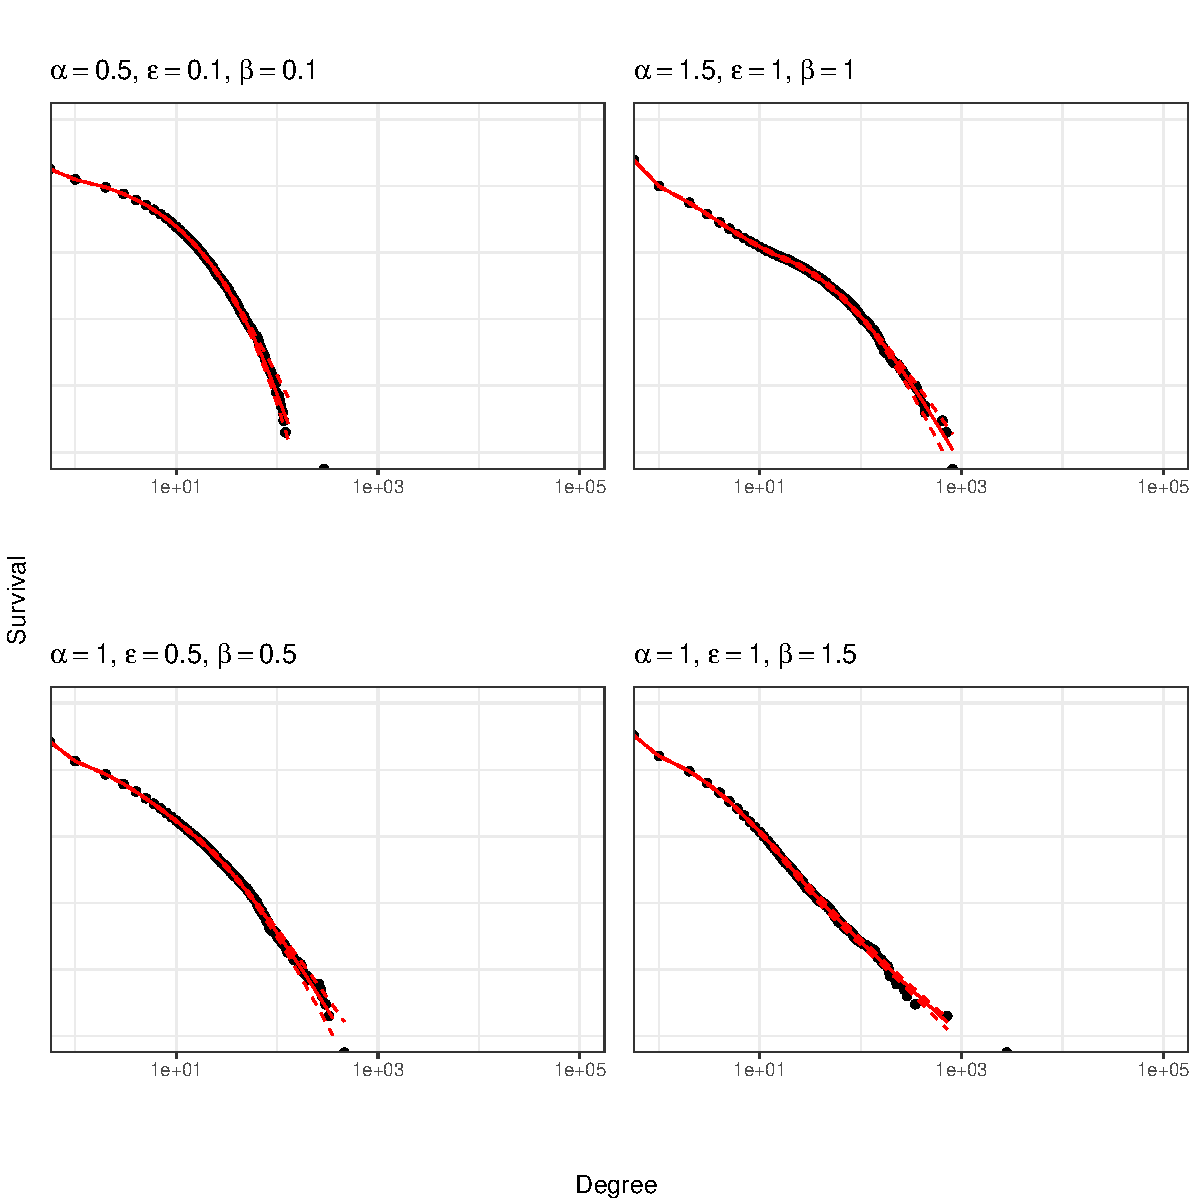
\includegraphics[width=0.8\linewidth,height=\textheight,keepaspectratio]{paper_files/figure-pdf/fig-rec1-1.pdf}

}

\caption{\label{fig-rec1}Posterior estimates of survival function for
data simulated from the proposed model with various combinations of
(\(\alpha\),\(\beta\),\(\varepsilon\)) and \(k_0=20\).}

\end{figure}%

\begin{figure}

\centering{

\pandocbounded{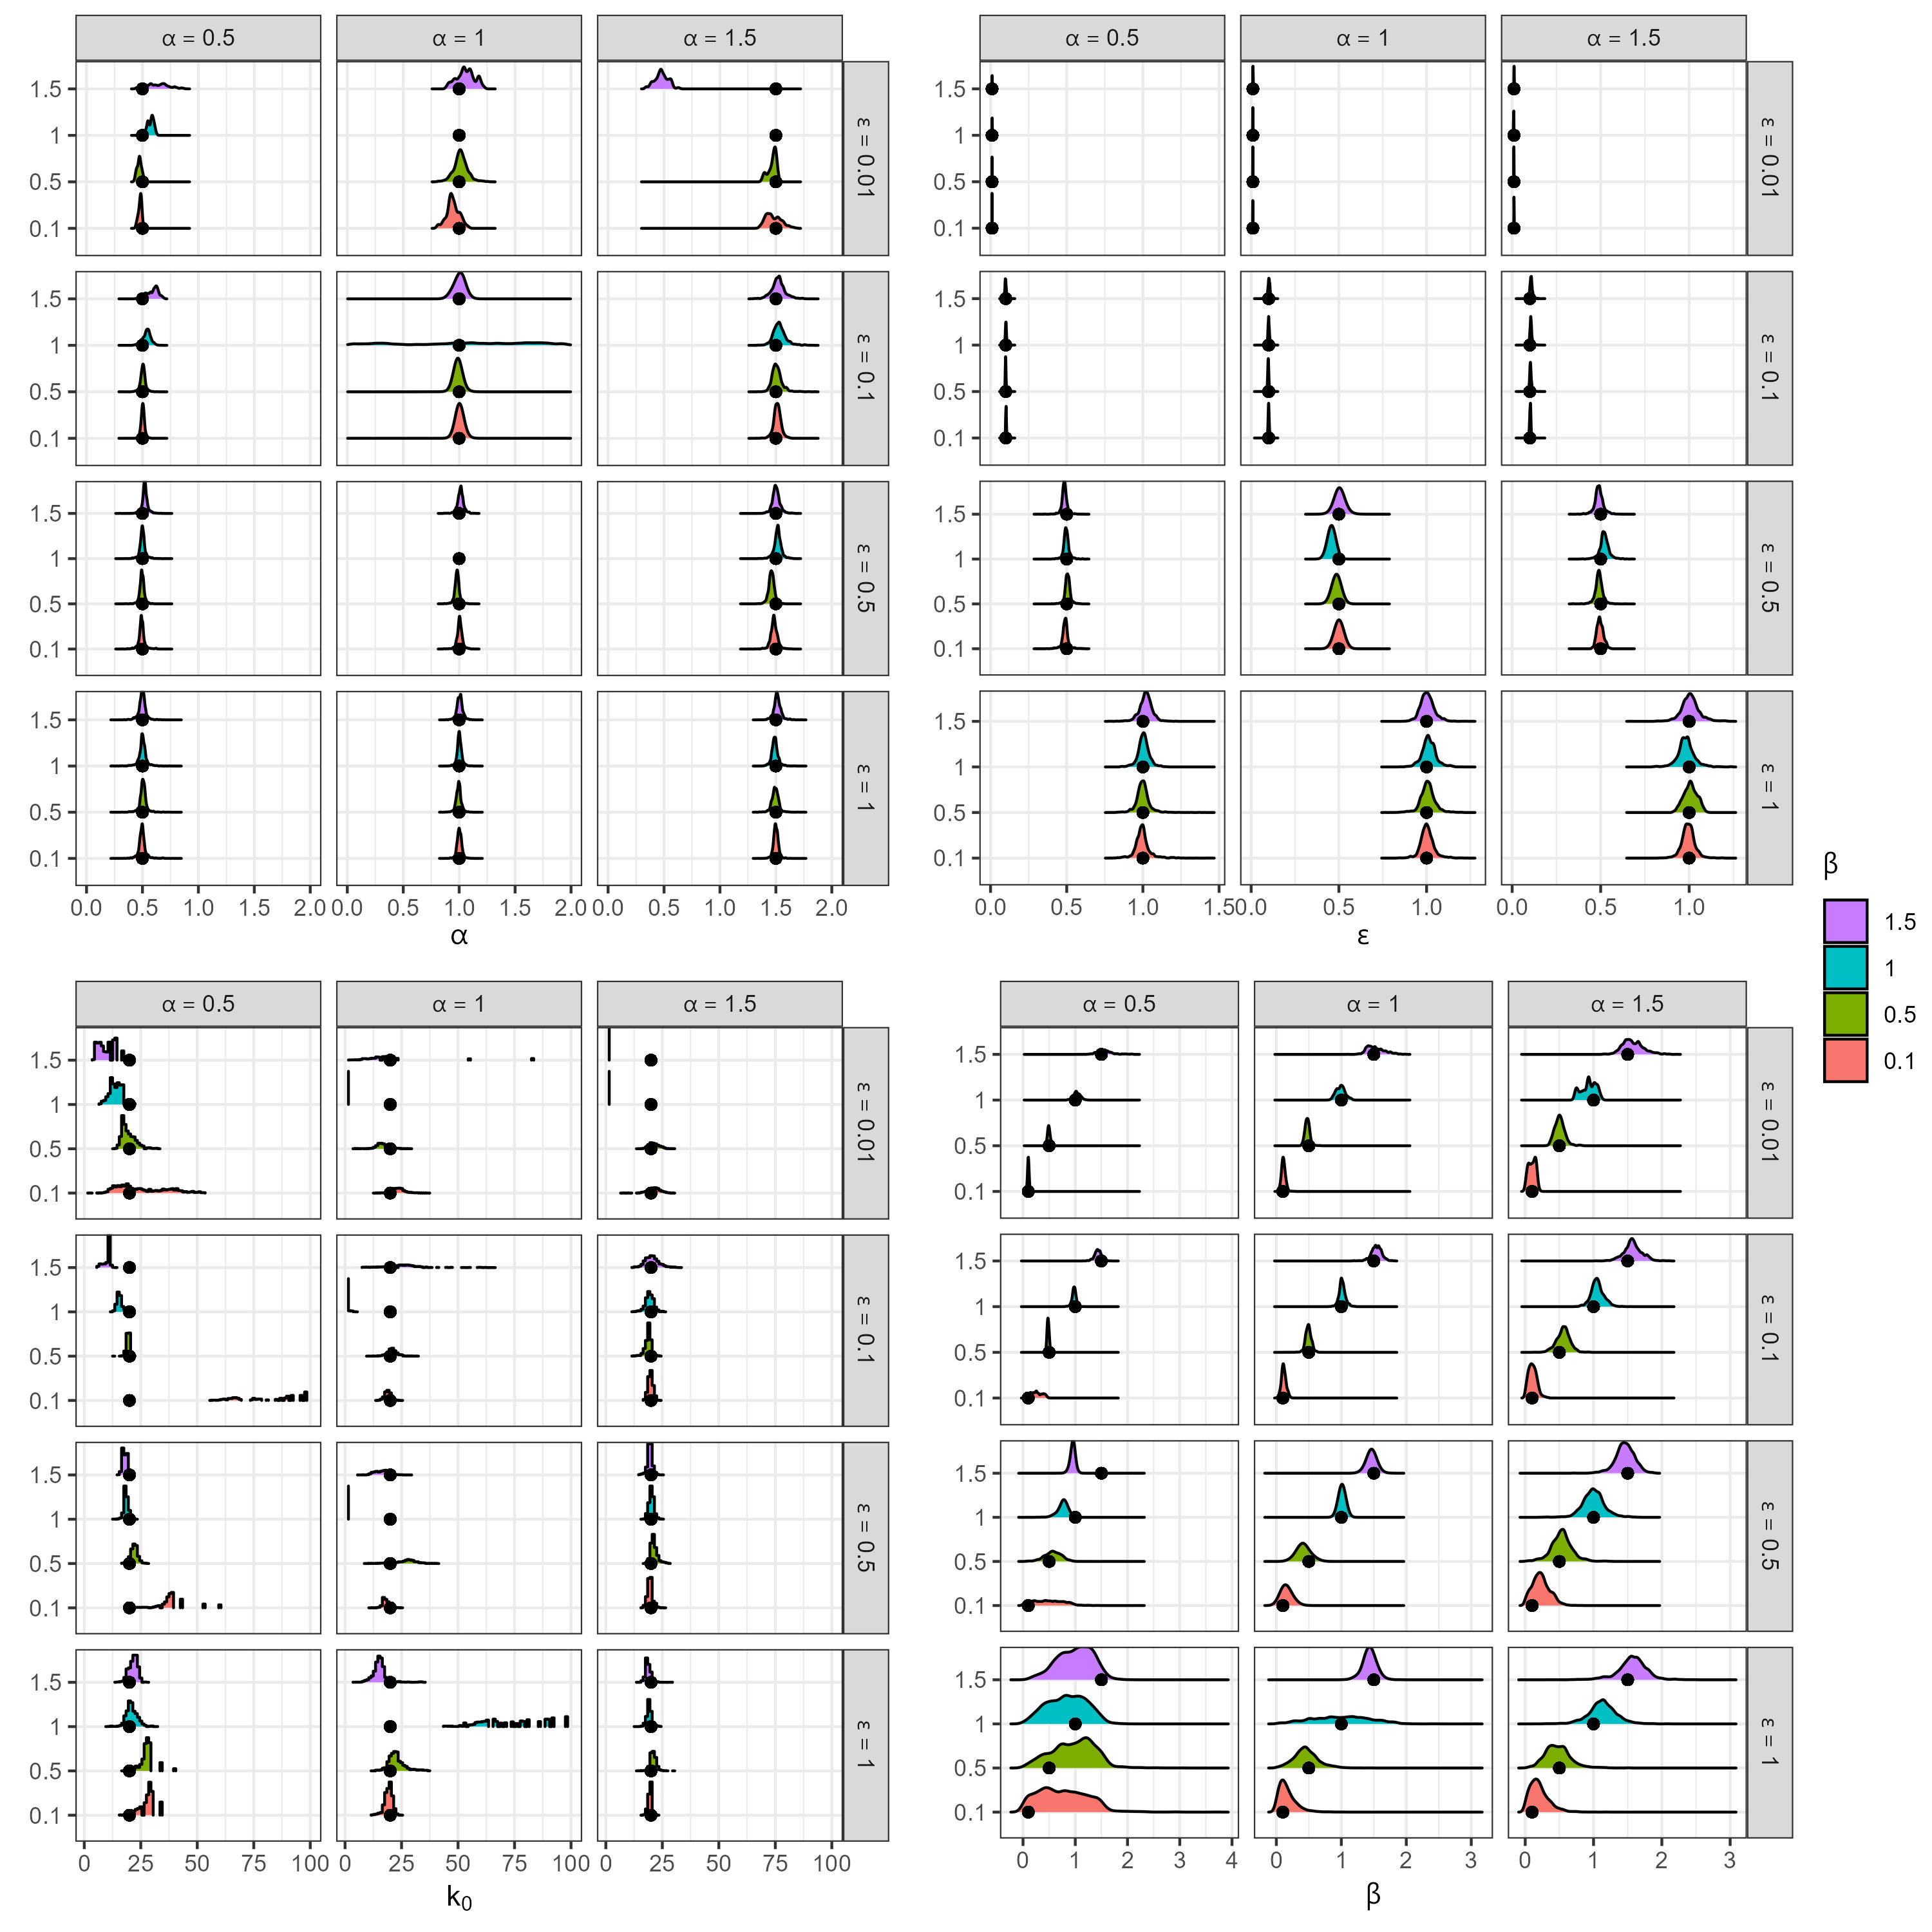
\includegraphics[keepaspectratio]{images/mcmc_plot.jpg}}

}

\caption{\label{fig-rec2}: Posterior estimates of paramters for data
simulated from the proposed model with various combinations of
(\(\alpha\),\(\beta\),\(\varepsilon\)) and \(k_0=20\).}

\end{figure}%

Figure~\ref{fig-rec1} and Figure~\ref{fig-rec2} shows the estimations
demonstrates that using this methodology it is possible to recover the
model parameters fairly well from only the final degree distribution of
a simulated network. This indicates that the method may also be able to
be applied to the degree distributions of real networks, estimating the
model parameters assuming they evolved according to the GPA scheme.

\section{Application to Real Data}\label{sec-real}

Turning now to real data, the goal is to fit the model to the degree
distributions of real networks from various sources and learn about the
mechanics of their growth. Alongside fitting this model to the degree
distributions, we then compare the fit to that of an mixture
distribution that was used in \citet{Lee24}, but this method has the
additional benefit of learning about a network's growth. The data
consists of 12 networks sourced from \href{konect.cc}{KONECT} and the
\href{https://networkrepository.com}{Network Data Repository}\citep{nr}:

\begin{itemize}
\tightlist
\item
  \texttt{as-caida20071105}: network of autonomous systems of the
  Internet connected with each other from the CAIDA project
\item
  \texttt{dimacs10-astro-ph} : co-authorship network from the
  ``astrophysics'' section (astro-ph) of arXiv
\item
  \texttt{ego-twitter}: network of twitter followers
\item
  \texttt{facebook-wosn-wall}: subset of network of Facebook wall pasts
\item
  \texttt{maayan-faa}: USA FAA (Federal Aviation Administration)
  preferred routes as recommended by the NFDC (National Flight Data
  Center)
\item
  \texttt{maayan-Stelzl}: network representing interacting pairs of
  proteins in Humans
\item
  \texttt{moreno-blogs-blogs}: network of URLs found on the first pages
  of individual blogs
\item
  \texttt{opsahl−openflights}: network containing flights between
  airports of the world.
\item
  \texttt{pajek-erdos}: co-authorship network around Paul Erdős
\item
  \texttt{reactome}: network of protein--protein interactions in Humans
\item
  \texttt{sx-mathoverflow}: interactions from the StackExchange site
  \href{https://mathoverflow.net/}{MathOverflow}
\item
  \texttt{topology}: network of connections between autonomous systems
  of the Internet
\end{itemize}

\begin{figure}

\centering{

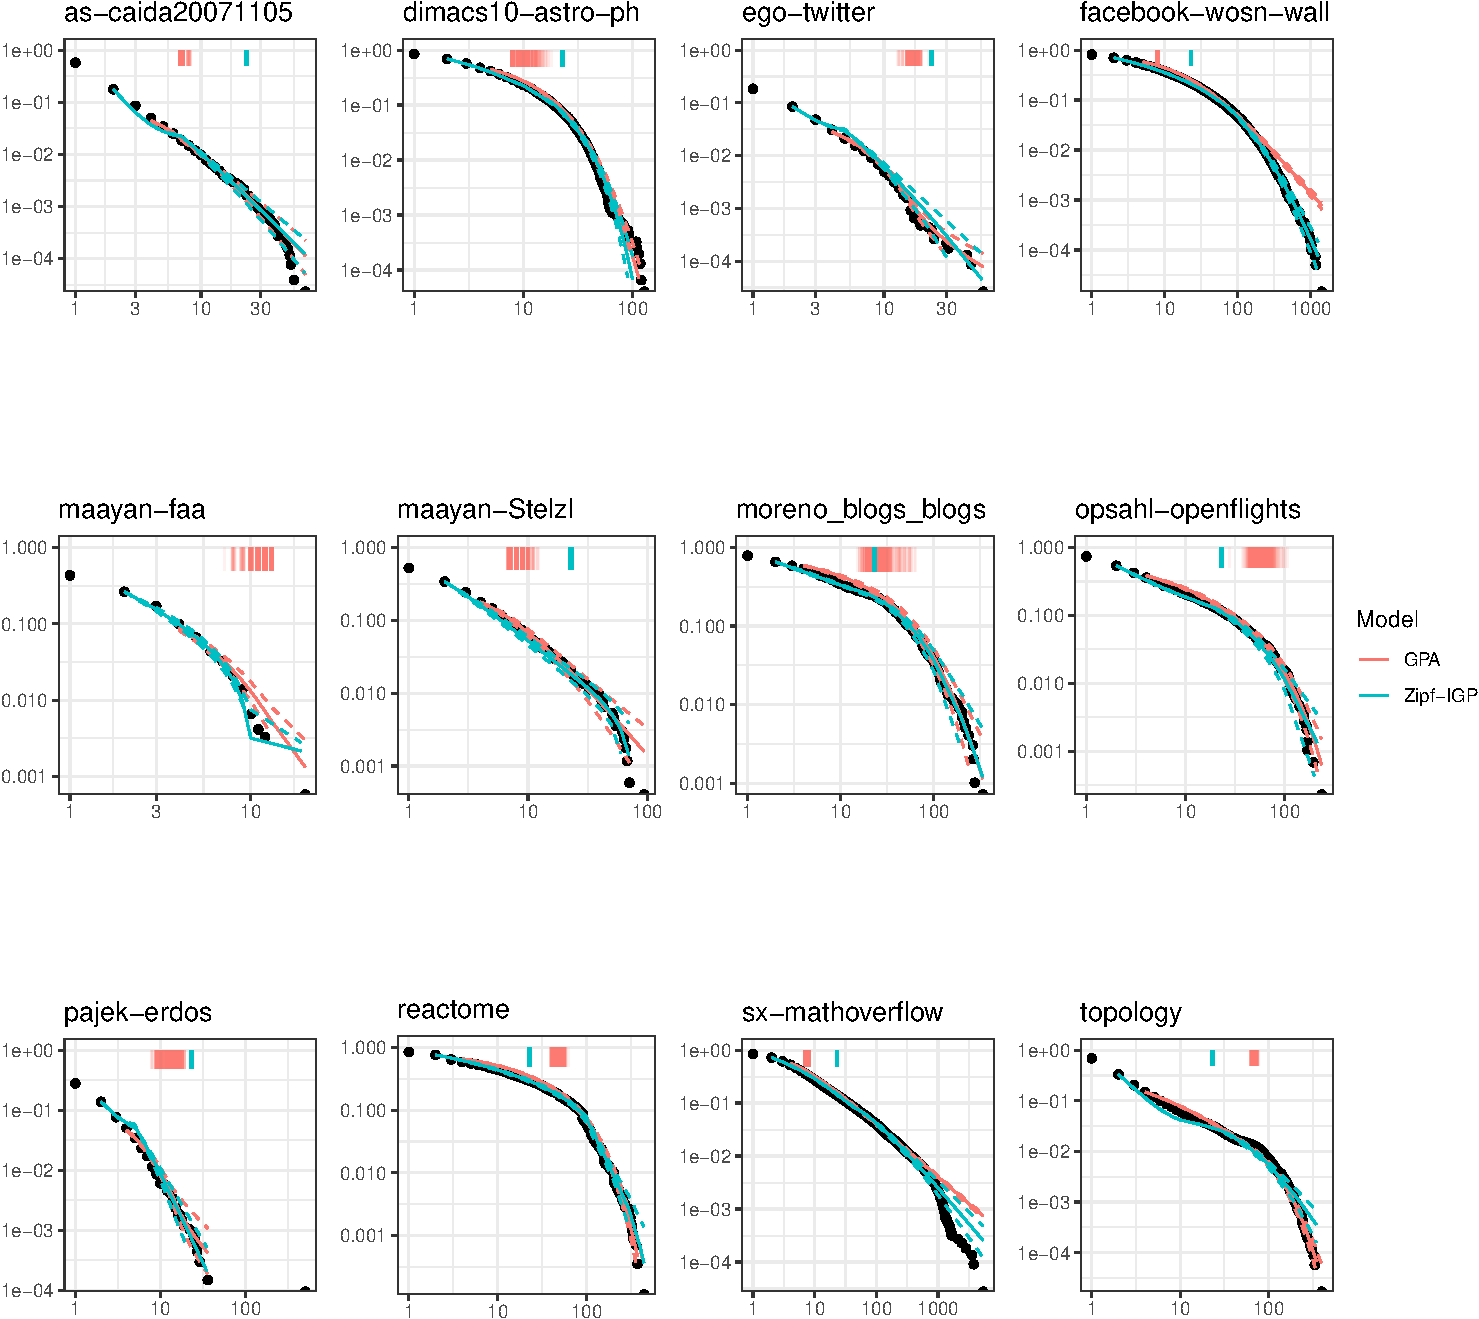
\includegraphics[width=0.8\linewidth,height=\textheight,keepaspectratio]{paper_files/figure-pdf/fig-real1-1.pdf}

}

\caption{\label{fig-real1}Posterior estimates (solid red) of survival
for several real data sets and their 95\% credible intervals (dotted
red)}

\end{figure}%

Figure~\ref{fig-real1} displays the posterior estimates of the survival
function for various data sets, obtained from fitting the GPA model and
the Zipf-IGP mixture model. In most cases, the GPA model does not
necessarily provide an improvement in fit when compared to the Zipf-IGP
model but where the GPA model fits well we gain additional information
about the preference function assuming that the network evolved
according the the GPA scheme. Figure~\ref{fig-shapes} shows the
posterior of the shape parameter \(\xi\) obtained from the Zipf-IGP
model alongside the posterior of the equivalent shape parameter
\(\beta/\lambda^*\) obtained from fitting the GPA model. Generally, the
GPA model performs similarly to the Zipf-IGP when estimating the tail
behaviour of the degree distribution and where it doesn't it appears to
either be because it is fitting better at the tail than the Zipf-IGP
model or because of the threshold being estimated as too low forcing
almost all of the data to be modelled by the linear part of the GPA.
This again shows the effects that small degrees have on this model,
which is somewhat expected as the theory used for this model is for
trees and none of these real networks (nor many real networks) are.

\begin{figure}

\centering{

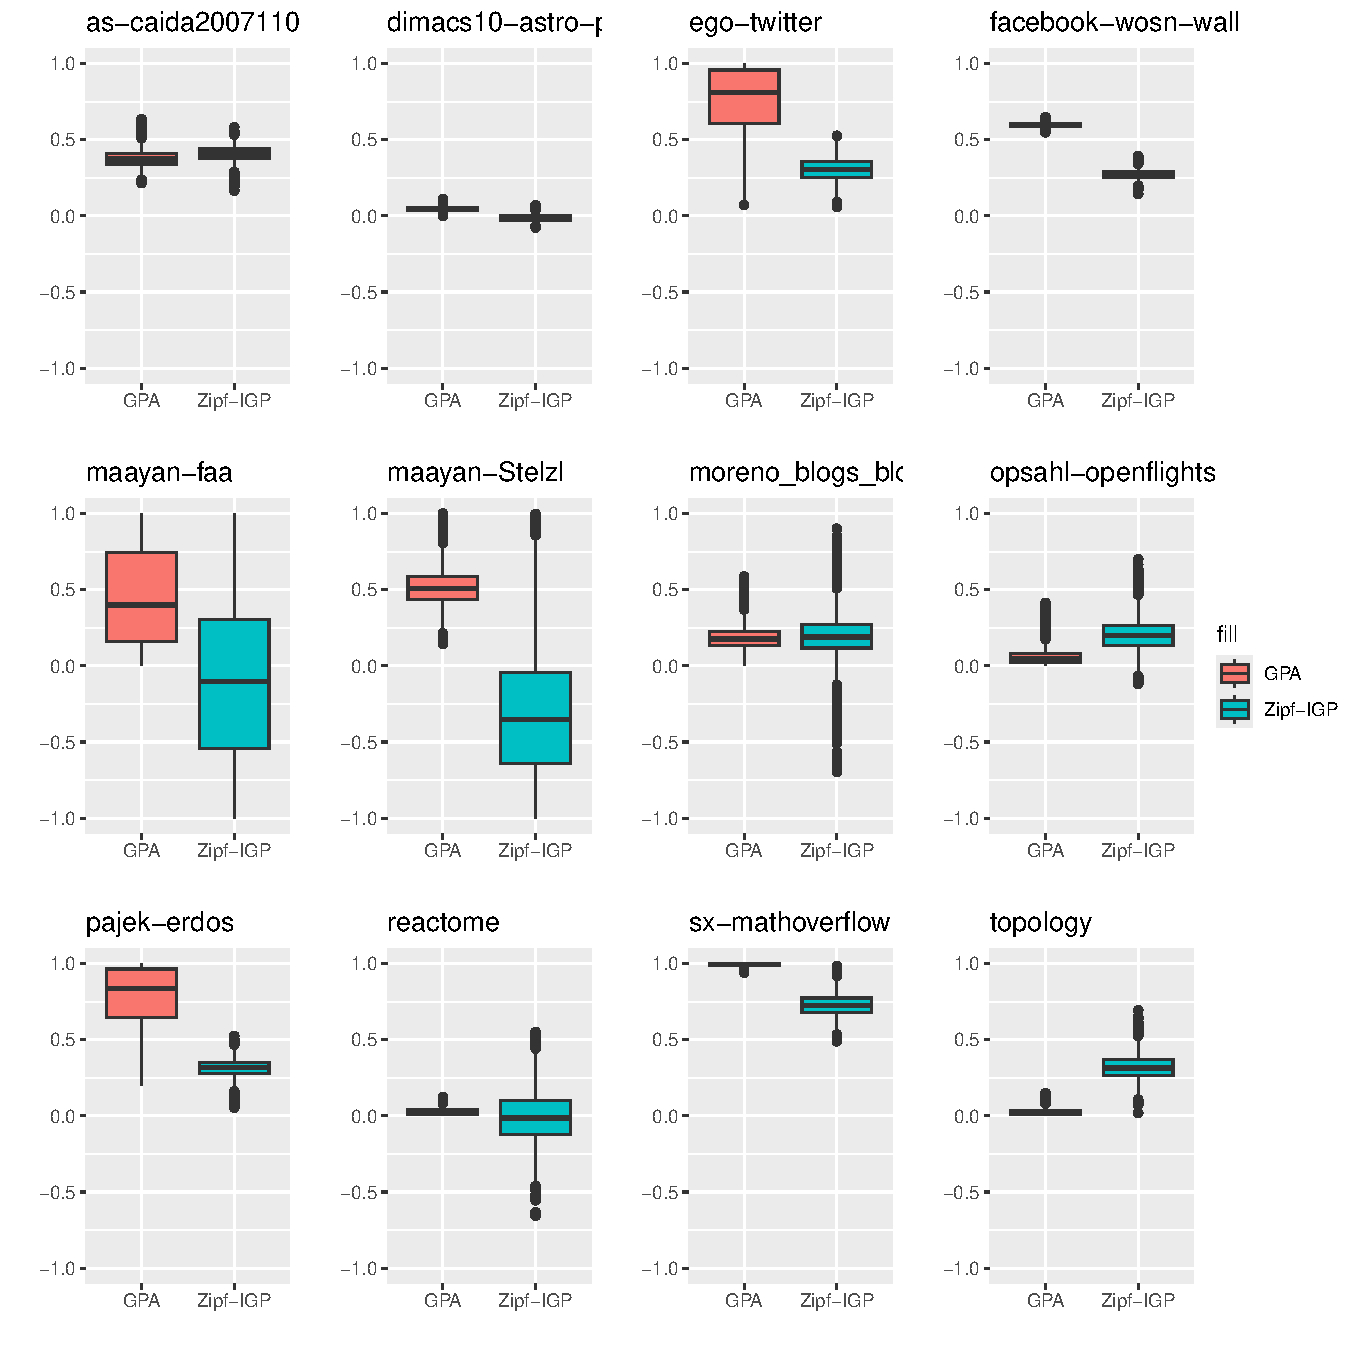
\includegraphics[width=0.8\linewidth,height=\textheight,keepaspectratio]{paper_files/figure-pdf/fig-shapes-1.pdf}

}

\caption{\label{fig-shapes}Posterior estimates (solid red) of survival
for several real data sets and their 95\% credible intervals (dotted
red)}

\end{figure}%

Figure~\ref{fig-pa} shows the estimated preference function \(b\)
alongside the 95\% credible interval on a log-log plot. Although the
credible interval becomes very large for the largest degrees, this is
expected as not all of these networks had data in that region, for those
that do the credible interval is much narrower as is the case for
\texttt{sx-mathoverflow}. The most insightful conclusion we can draw
from these plots come from the shape of the preference function. There
appears to be two distinct shapes of preference function. The first
appears mostly flat (similar to UA) for the smallest degrees and then
after a threshold PA kicks in, some with this shape are
\texttt{pajek-erdos} and \texttt{sx-mathoverflow}, maybe suggesting that
most vertices are just as liekly to gain connections as each other but
after gaining a number of connections become much more attractive
gaining more influence based on the number of connections they have. The
second distinct shape appears provide some clear PA behaviour that then
slows down after a certain point, examples of this are seen in the two
infrastructure networks \texttt{opsahl-openflights} and
\texttt{topology}. This slowing down could be viewed as a kind of
diminishing returns on the degree of a vertex i.e.~as a vertex gets
larger gaining more connections has less of an effect than it did before
some threshold \(k_0\).

\begin{figure}

\centering{

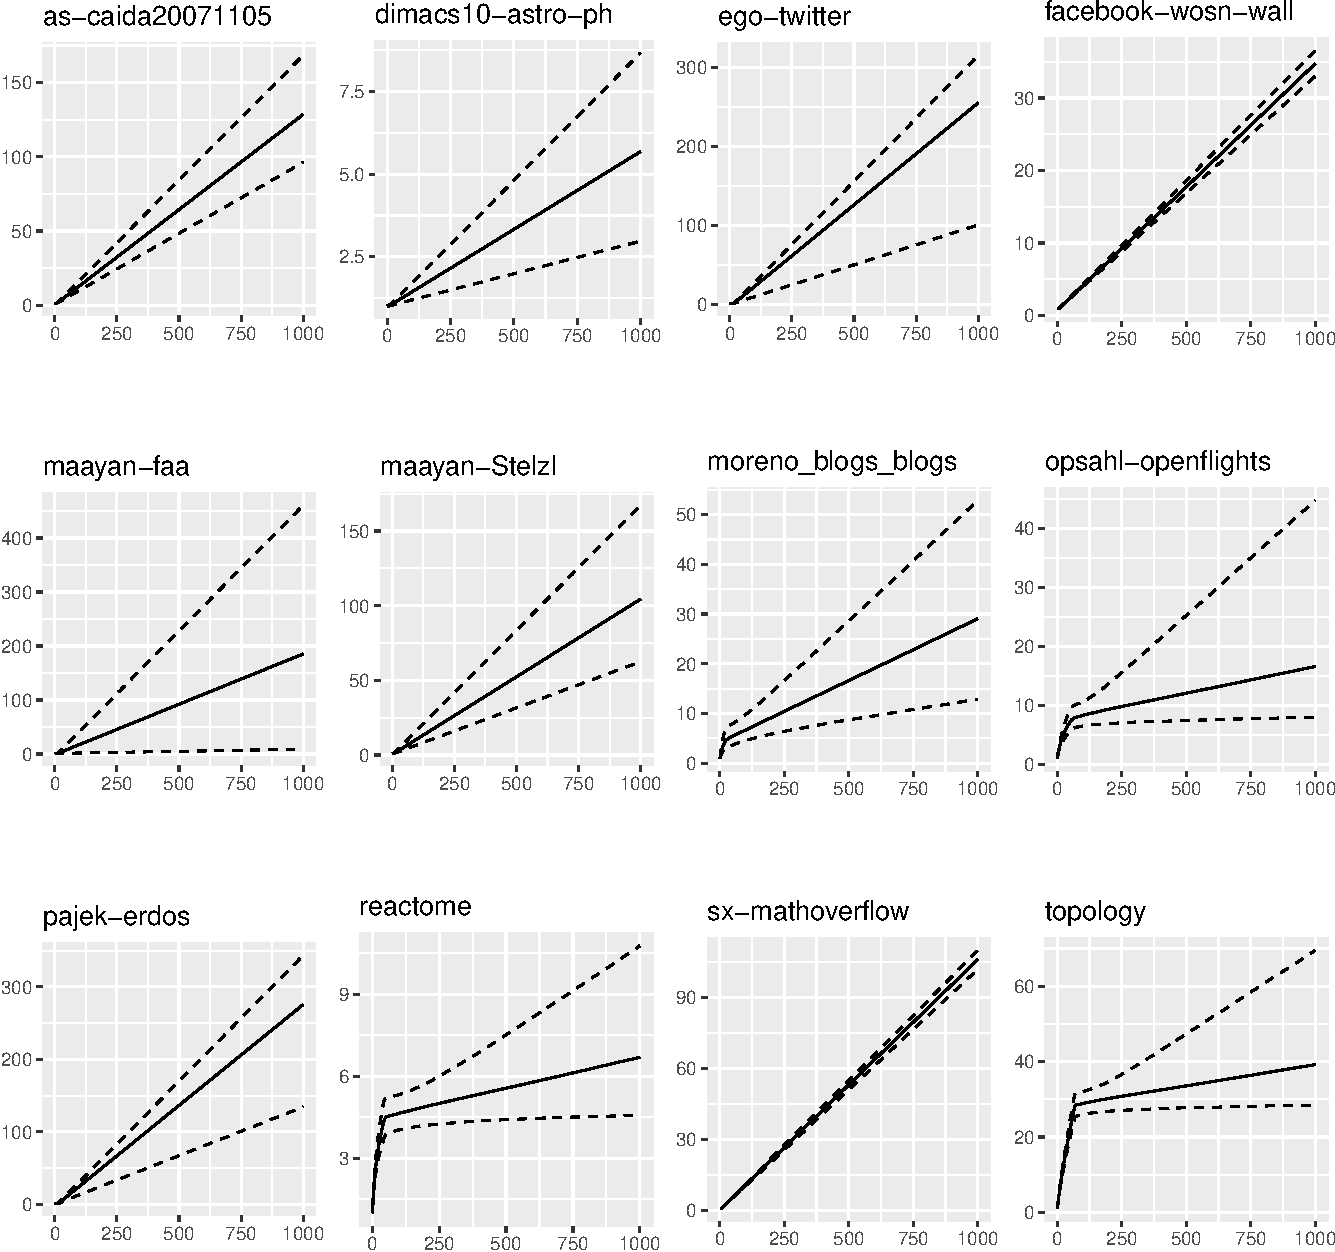
\includegraphics[width=0.8\linewidth,height=\textheight,keepaspectratio]{paper_files/figure-pdf/fig-pa-1.pdf}

}

\caption{\label{fig-pa}Posterior estimate for preference function
(solid) with 95\% credible interval (dashed) on log-log scale.}

\end{figure}%

\begin{figure}[H]

{\centering \pandocbounded{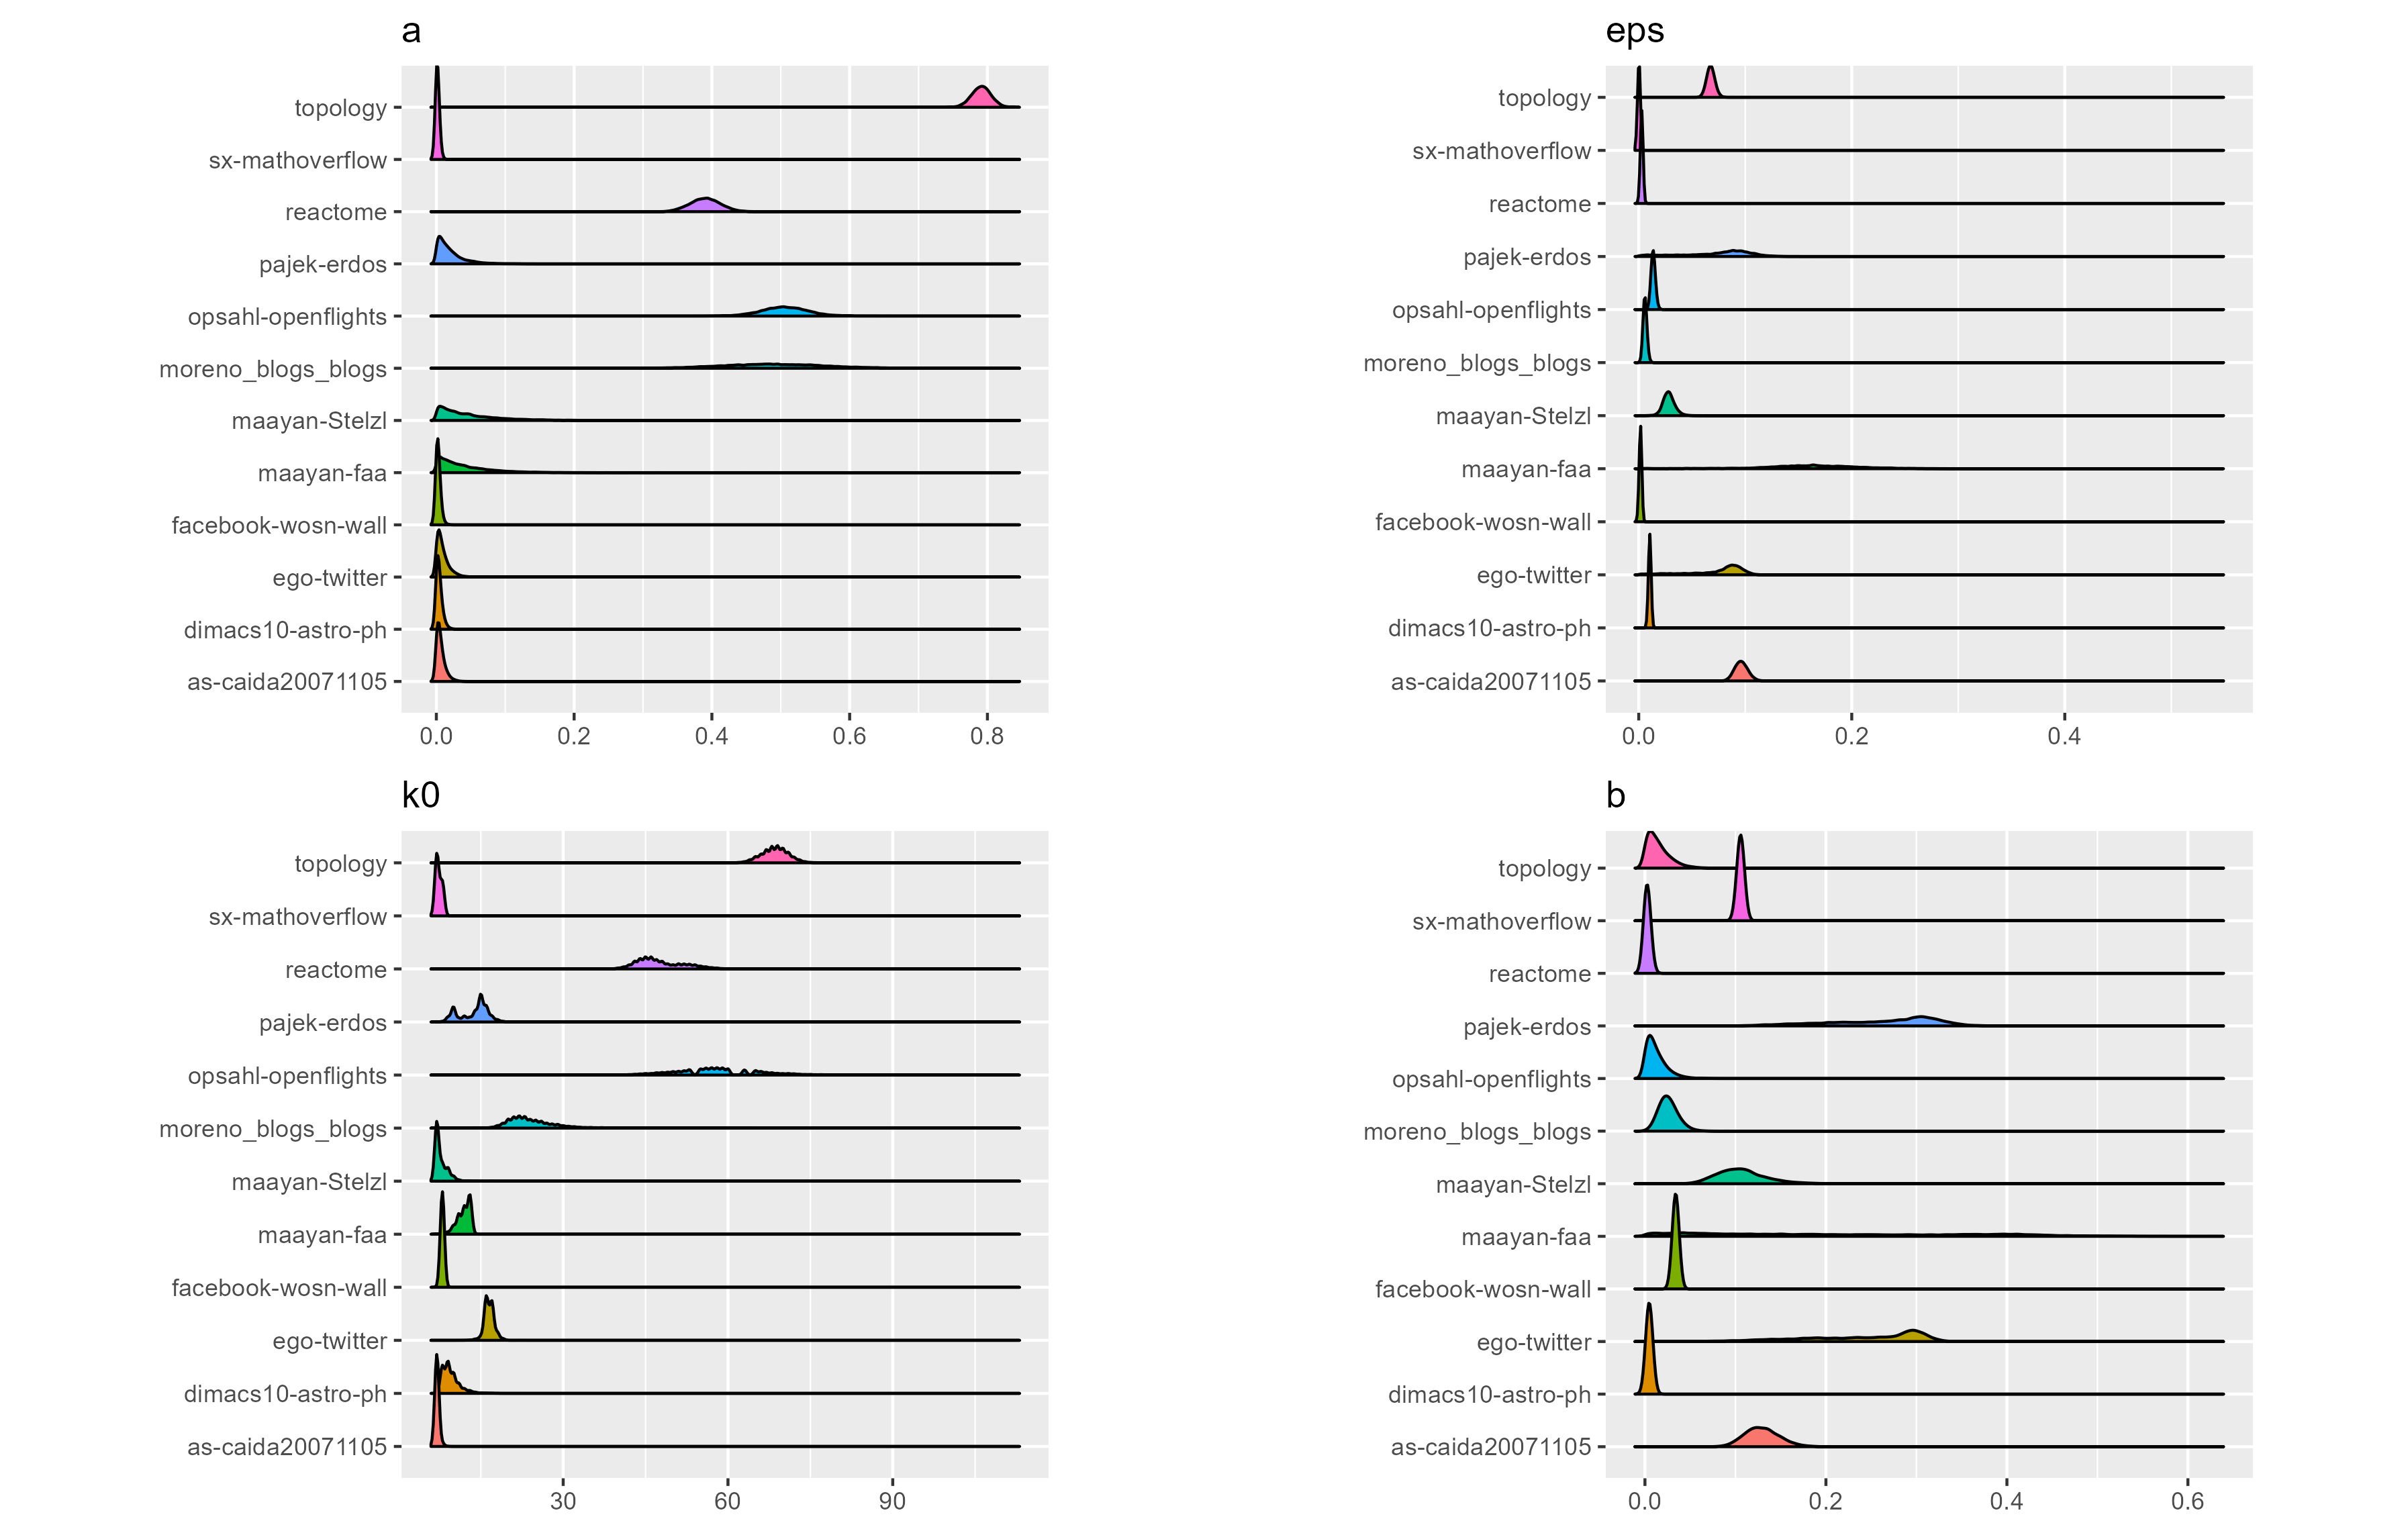
\includegraphics[keepaspectratio]{images/pars_plot.png}}

}

\caption{: Posterior estimates of paramters for real data.}

\end{figure}%

\section{Conclusion and Discussion}\label{conclusion-and-discussion}

In this paper we introduced a flexible class of preference function that
when used under the GPA scheme (in the tree setting) is guaranteed to
generate a network with a heavy tailed degree distribution whilst
remaining flexible in the body. Using simulations from networks using
this class of preference function we showed that the model parameters
are quite easily estimated from the degrees alone at a snapshot in time.
Seeing this we applied this method to the degree distributions of real
networks, estimating their model parameters assuming they evolved in the
same way. Not only did this yield fairly good fits for the degree
distribution, similar to that of the Zipf-IGP, it came with the added
benefit of giving a posterior estimate for a preference function.

One limitation of this method is that the lowest degrees needed to be
truncated as they had a very large effect on the fit of the model as a
result of using theory developed for trees and applying it to general
networks. Future work could apply theory developed for general networks
using a similar method to this, allowing us to compare the results here
something that is more accurate.

\setcounter{section}{0}
\renewcommand{\thesection}{\Alph{section}}
\setcounter{table}{0}
\renewcommand{\thetable}{A\arabic{table}}
\setcounter{figure}{0}
\renewcommand{\thefigure}{A\arabic{figure}}

\newpage

\section{Proofs and Derivations}\label{sec-proofs}

\subsection{\texorpdfstring{Proof of
Proposition~\ref{prp-omega}}{Proof of Proposition~}}\label{proof-of-prp-omega}

Taking the form of the GPA degree survival: \[
\bar F(n) = \prod_{i=0}^n\frac{b(i)}{\lambda+b(i)}
\] and substituting into the formula for \(\Omega(F,n)\):

\begin{align*}
\Omega(F,n)&=\left(\log\frac{\prod_{i=0}^{n+1}\frac{b(i)}{\lambda+b(i)}}{\prod_{i=0}^{n+2}\frac{b(i)}{\lambda+b(i)}}\right)^{-1}-\left(\log\frac{\prod_{i=0}^{n}\frac{b(i)}{\lambda+b(i)}}{\prod_{i=0}^{n+1}\frac{b(i)}{\lambda+b(i)}}\right)^{-1}\\
&=\left(\log\frac{\lambda+b(n+2)}{b(n+2)}\right)^{-1}-\left(\log\frac{\lambda+b(n+1)}{b(n+1)}\right)^{-1}\\
&=\left(\log\left[1+\frac{\lambda}{b(n+2)}\right]\right)^{-1}-\left(\log\left[1+\frac{\lambda}{b(n+1)}\right]\right)^{-1}
\end{align*}

Clearly if \(b(n)=c\) or \(\lim_{n\rightarrow\infty}b(n)=c\) for some
\(c>0\) then \(\Omega(F,n)=0\). Now consider a non-constant \(b(n)\) and
re-write \(\Omega(F,n)\) as:

\begin{align*}
\Omega(F,n) &= \left(\log\left[1+\frac{\lambda}{b(n+2)}\right]\right)^{-1}-\frac{b(n+2)}{\lambda}+\frac{b(n+2)}{\lambda}-\left(\log\left[1+\frac{\lambda}{b(n+1)}\right]\right)^{-1}\\&+\frac{b(n+1)}{\lambda}  -\frac{b(n+1)}{\lambda}\\
&=\left\{ \left(\log\left[1+\frac{\lambda}{b(n+2)}\right]\right)^{-1}-\frac{b(n+2)}{\lambda}\right\} - \left\{ \left(\log\left[1+\frac{\lambda}{b(n+1)}\right]\right)^{-1}-\frac{b(n+1)}{\lambda}\right\}\\&+\frac{b(n+2)}{\lambda}-\frac{b(n+1)}{\lambda}
\end{align*}

Then if \(\lim_{n\rightarrow\infty}b(n)=\infty\) it follows that:

\begin{align*}
\lim_{n\rightarrow\infty}\Omega(F,n) &= \lim_{n\rightarrow\infty}\left\{ \left(\log\left[1+\frac{\lambda}{b(n+2)}\right]\right)^{-1}-\frac{b(n+2)}{\lambda}\right\} \\&- \lim_{n\rightarrow\infty}\left\{ \left(\log\left[1+\frac{\lambda}{b(n+1)}\right]\right)^{-1}-\frac{b(n+1)}{\lambda}\right\}\\
&\qquad+\lim_{n\rightarrow\infty}\left(\frac{b(n+2)}{\lambda}-\frac{b(n+1)}{\lambda}\right)\\
&=\frac{1}{2}-\frac{1}{2} + \lim_{n\rightarrow\infty}\left(\frac{b(n+2)}{\lambda}-\frac{b(n+1)}{\lambda}\right)\\
&=\frac{1}{\lambda}\lim_{n\rightarrow\infty}\left[b(n+2)-b(n+1)\right]\qquad \square
\end{align*}

\subsection{\texorpdfstring{Derivation of
Equation~\ref{eq-rho}}{Derivation of Equation~}}\label{derivation-of-eq-rho}

For a preference function of the form:

\[
b(k) = \begin{cases}
g(k),&k<k_0\\
g(k_0) + \beta(k-k_0), &k\ge k_0
\end{cases}
\] for \(\beta>0, k_0\in\mathbb N\) we have that

\begin{align*}
\hat\rho(\lambda) = \sum_{n=0}^\infty\prod_{i=0}^{n-1}\frac{b(i)}{\lambda+b(i)} &= \sum_{n=0}^{k_0}\prod_{i=0}^{n-1}\frac{g(i)}{\lambda+g(i)} + \sum_{n=k_0+1}^\infty\left(\prod_{i=0}^{k_0-1}\frac{g(i)}{\lambda+g(i)}\prod_{i=k_0}^{n-1}\frac{g(k_0) + \beta(i-k_0)}{\lambda +g(k_0) + \beta(i-k_0)}\right)\\
&=\sum_{n=0}^{k_0}\prod_{i=0}^{n-1}\frac{g(i)}{\lambda+g(i)} + \left(\prod_{i=0}^{k_0-1}\frac{g(i)}{\lambda+g(i)}\right)\sum_{n=k_0+1}^\infty\prod_{i=k_0}^{n-1}\frac{g(k_0) + \beta(i-k_0)}{\lambda +g(k_0) + \beta(i-k_0)}
\end{align*}

Now using the fact that:

\[
\prod_{i=0}^n(x+yi) = x^{n+1}\frac{\Gamma(\frac{x}{y}+n+1)}{\Gamma(\frac{x}{y})}
\] and reindexing the product in the second sum

\begin{align*}
\hat\rho(\lambda) &= \sum_{n=0}^{k_0}\prod_{i=0}^{n-1}\frac{g(i)}{\lambda+g(i)} + \left(\prod_{i=0}^{k_0-1}\frac{g(i)}{\lambda+g(i)}\right)\sum_{n=k_0+1}^\infty\frac{\Gamma\left(\frac{g(k_0)}{\beta}+n-k_0\right)\Gamma\left(\frac{\lambda+g(k_0)}{\beta}\right)}{\Gamma\left(\frac{\lambda+g(k_0)}{\beta}+n-k_0\right)\Gamma\left(\frac{g(k_0)}{\beta}\right)}\\
&= \sum_{n=0}^{k_0}\prod_{i=0}^{n-1}\frac{g(i)}{\lambda+g(i)} + \frac{\Gamma\left(\frac{\lambda+g(k_0)}{\beta}\right)}{\Gamma\left(\frac{g(k_0)}{\beta}\right)}\left(\prod_{i=0}^{k_0-1}\frac{g(i)}{\lambda+g(i)}\right)\sum_{n=k_0+1}^\infty\frac{\Gamma\left(\frac{g(k_0)}{\beta}+n-k_0\right)}{\Gamma\left(\frac{\lambda+g(k_0)}{\beta}+n-k_0\right)}\\
&=\sum_{n=0}^{k_0}\prod_{i=0}^{n-1}\frac{g(i)}{\lambda+g(i)} + \frac{\Gamma\left(\frac{\lambda+g(k_0)}{\beta}\right)}{\Gamma\left(\frac{g(k_0)}{\beta}\right)}\left(\prod_{i=0}^{k_0-1}\frac{g(i)}{\lambda+g(i)}\right)\sum_{n=1}^\infty\frac{\Gamma\left(\frac{g(k_0)}{\beta}+n\right)}{\Gamma\left(\frac{\lambda+g(k_0)}{\beta}+n\right)}
\end{align*}

In order to simplify the infinite sum, consider:

\begin{align*}
\sum_{n=0}^\infty\frac{\Gamma(n+x)}{\Gamma(n+x+y)} &=\frac{1}{\Gamma(y)}\sum_{n=0}^\infty \text{B}(n+x,y)\\
&=\frac{1}{\Gamma(y)}\sum_{n=0}^\infty\int_0^1t^{n+x-1}(1-t)^{y-1}at\\
&=\frac{1}{\Gamma(y)}\int_0^1 t^{x-1}(1-t)^{y-1}\sum_{n=0}^\infty t^n\,at\\
&=\frac{1}{\Gamma(y)}\int_0^1 t^{x-1}(1-t)^{y-1}\frac{1}{1-t}at\\
&=\frac{1}{\Gamma(y)}\int_0^1 t^{x-1}(1-t)^{y-2}at\\
&=\frac{1}{\Gamma(y)}\text{y}(x,y-1)\\
&= \frac{\Gamma(x)}{(y-1)\Gamma(x+y-1)}
\end{align*}

this infinite sum does not converge when \(x\le1\) as each term is
\(O(n^{-x})\). We can now use this in \(\hat\rho(\lambda)\):

\begin{align*}
\hat\rho(\lambda) &= \sum_{n=0}^{k_0}\prod_{i=0}^{n-1}\frac{g(i)}{\lambda+g(i)} + \frac{\Gamma\left(\frac{\lambda+g(k_0)}{\beta}\right)}{\Gamma\left(\frac{g(k_0)}{\beta}\right)}\left(\prod_{i=0}^{k_0-1}\frac{g(i)}{\lambda+g(i)}\right)\left(\frac{\Gamma\left(\frac{g(k_0)}{\beta}\right)}{\left(\frac{\lambda}{\beta}-1\right)\Gamma\left(\frac{g(k_0)+\lambda}{\beta}-1\right)}-\frac{\Gamma\left(\frac{g(k_0)}{\beta}\right)}{\Gamma\left(\frac{g(k_0)+\lambda}{\beta}\right)}\right)\\
&=\sum_{n=0}^{k_0}\prod_{i=0}^{n-1}\frac{g(i)}{\lambda+g(i)} + \left(\prod_{i=0}^{k_0-1}\frac{g(i)}{\lambda+g(i)}\right)\left(\frac{\Gamma\left(\frac{g(k_0)+\lambda}{\beta}\right)}{\left(\frac{\lambda}{\beta}-1\right)\Gamma\left(\frac{g(k_0)+\lambda}{\beta}-1\right)}-1\right)\\
&=\sum_{n=0}^{k_0}\prod_{i=0}^{n-1}\frac{g(i)}{\lambda+g(i)} + \left(\prod_{i=0}^{k_0-1}\frac{g(i)}{\lambda+g(i)}\right)\left(\frac{\frac{g(k_0)+\lambda}{\beta}-1}{\frac{\lambda}{\beta}-1}-1\right)\\
&=\sum_{n=0}^{k_0}\prod_{i=0}^{n-1}\frac{g(i)}{\lambda+g(i)} + \left(\prod_{i=0}^{k_0-1}\frac{g(i)}{\lambda+g(i)}\right)\left(\frac{g(k_0)+\lambda-\beta}{\lambda-\beta}-1\right)\\&=\sum_{n=0}^{k_0}\prod_{i=0}^{n-1}\frac{g(i)}{\lambda+g(i)} + \frac{g(k_0)}{\lambda-\beta}\prod_{i=0}^{k_0-1}\frac{g(i)}{\lambda+g(i)}\qquad \square
\end{align*}

\newpage

\section{Additional Tables and
Figures}\label{additional-tables-and-figures}

\newpage

\section*{References}\label{references}
\addcontentsline{toc}{section}{References}

\renewcommand{\bibsection}{}
\bibliography{refs.bib}





\end{document}
